\chapter{Thực nghiệm và kết quả}

\section{Thiết lập thực nghiệm}
Thí nghiệm baseline được chạy trên train = 7.664 mẫu, validation = 1.352 mẫu và held-out test = 500 mẫu. Tất cả mục tiêu đánh giá dùng cùng \code{label_target}. Baseline BoW/TF--IDF/Word2Vec sử dụng seed 42; Word2Vec Skip-gram chạy một worker để tăng khả năng tái lập. Macro-F1 được chọn làm chỉ số chính. Khoảng tin cậy percentile 95\% được ước lượng bằng 1.000 bootstrap resamples trên dự đoán test.

\section{Kết quả tổng hợp}
Bảng \ref{tab:leaderboard} cho thấy Word2Vec + LinearSVC có Macro-F1 test cao nhất trong các baseline đã chạy (0,6949), sát với BoW + MultinomialNB (0,6790). Majority baseline đạt Accuracy 0,640 nhưng Macro-F1 chỉ 0,2602 do không nhận diện hai lớp thiểu số. TF--IDF + LinearSVC có Accuracy cao nhất (0,830) nhưng Macro-F1 là 0,6626, thấp hơn Word2Vec + LinearSVC; điều này minh họa vì sao Accuracy không nên là tiêu chí duy nhất khi lớp bị mất cân bằng.

\begin{table}[H]
\centering
\caption{So sánh baseline trên held-out pseudo-labeled test}
\label{tab:leaderboard}
\small
\resizebox{\textwidth}{!}{%
\begin{tabular}{lrrrrrr}
\toprule
Mô hình & Accuracy & Macro-P & Macro-R & Macro-F1 & Weighted-F1 & Bootstrap CI 95\% (Macro-F1) \\
\midrule
Majority baseline & 0,640 & 0,2133 & 0,3333 & 0,2602 & 0,4995 & [0,2490; 0,2703] \\
BoW + MultinomialNB & 0,814 & 0,6742 & 0,6878 & 0,6790 & 0,8136 & [0,6305; 0,7270] \\
BoW + LinearSVC & 0,818 & 0,6906 & 0,6576 & 0,6632 & 0,8022 & [0,6144; 0,7100] \\
TF--IDF + MultinomialNB & 0,818 & 0,6578 & 0,6500 & 0,6378 & 0,7999 & [0,5936; 0,6881] \\
TF--IDF + LinearSVC & 0,830 & 0,6827 & 0,6688 & 0,6626 & 0,8130 & [0,6182; 0,7116] \\
Word2Vec + GaussianNB & 0,736 & 0,6060 & 0,6392 & 0,6119 & 0,7567 & [0,5703; 0,6593] \\
\textbf{Word2Vec + LinearSVC} & \textbf{0,828} & \textbf{0,6941} & \textbf{0,7038} & \textbf{0,6949} & \textbf{0,8246} & [0,6467; 0,7445] \\
\bottomrule
\end{tabular}}
\end{table}

\begin{figure}[H]
  \centering
  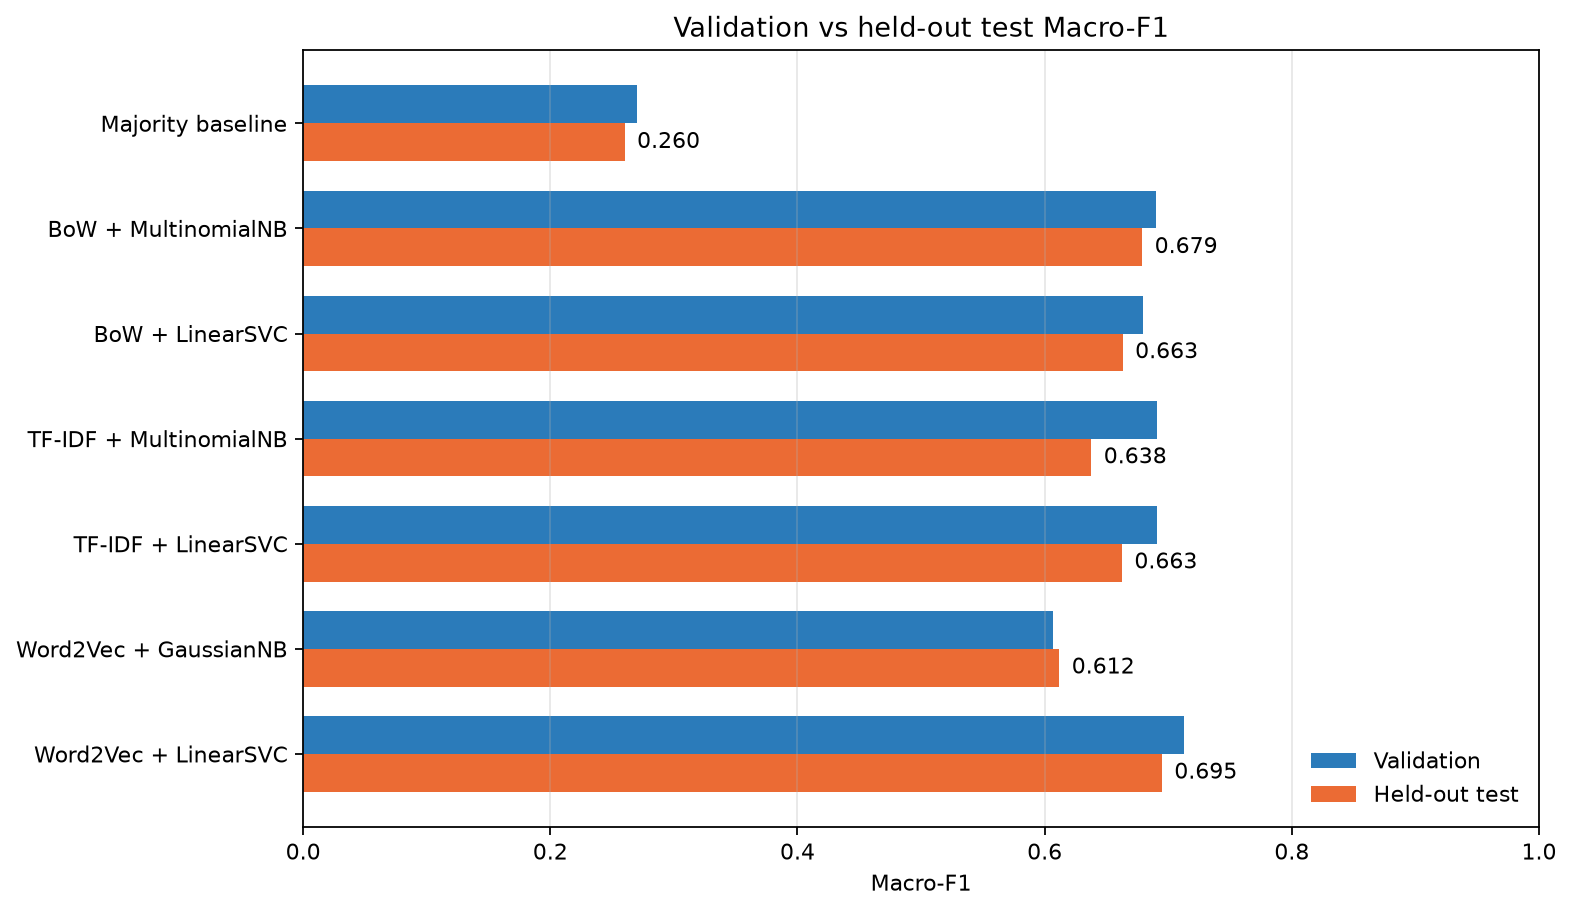
\includegraphics[width=0.92\textwidth]{macro_f1_val_test.png}
  \caption{Macro-F1 của các baseline trên validation và held-out test. Cả hai split sử dụng cùng nhãn đích hybrid.}
  \label{fig:macro-f1}
\end{figure}

\begin{figure}[H]
  \centering
  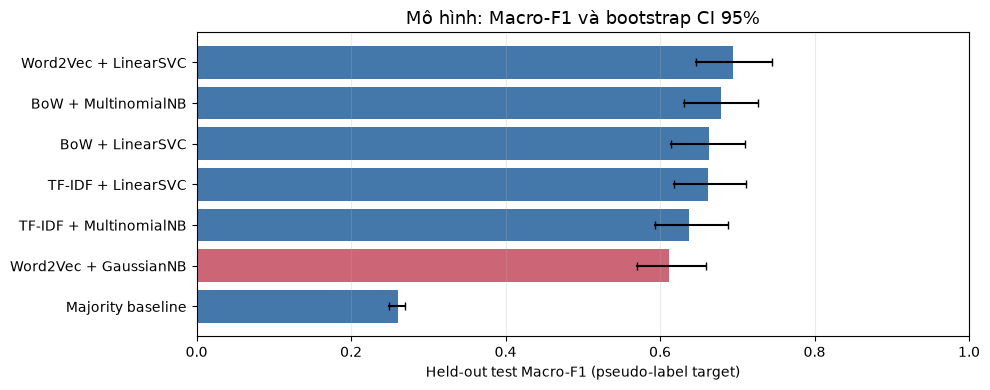
\includegraphics[width=0.90\textwidth]{macro_f1_test_ci.png}
  \caption{Macro-F1 trên held-out test kèm bootstrap CI 95\%. Các khoảng chồng lấp nên chênh lệch nhỏ cần được diễn giải thận trọng.}
  \label{fig:macro-f1-ci}
\end{figure}

Khoảng tin cậy giữa các mô hình có phần chồng lấp. Vì vậy, không kết luận chênh lệch nhỏ giữa các baseline là có ý nghĩa thống kê; kết quả cần được xác nhận bằng lặp seed/cross-validation và đặc biệt là nhãn được người gán độc lập.

\section{Phân tích theo lớp}
\begin{table}[H]
\centering
\caption{Chỉ số từng lớp của Word2Vec + LinearSVC}
\label{tab:per-class}
\begin{tabular}{lrrrr}
\toprule
Lớp & Precision & Recall & F1-score & Support \\
\midrule
Negative & 0,7241 & 0,8750 & 0,7925 & 120 \\
Neutral & 0,4167 & 0,3333 & 0,3704 & 60 \\
Positive & 0,9414 & 0,9031 & 0,9219 & 320 \\
\bottomrule
\end{tabular}
\end{table}

\begin{figure}[H]
  \centering
  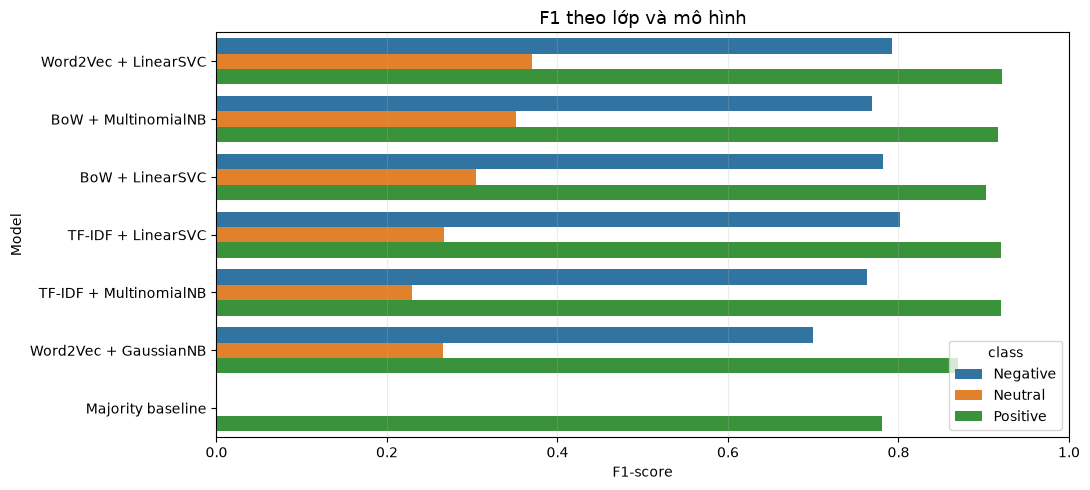
\includegraphics[width=0.93\textwidth]{per_class_f1_models.png}
  \caption{F1-score theo từng lớp và mô hình. Biểu đồ cho thấy hiệu năng lớp Neutral thường thấp hơn các lớp còn lại.}
  \label{fig:per-class-f1}
\end{figure}

Mô hình nhận diện tốt lớp Positive và Negative theo pseudo-label, nhưng lớp Neutral yếu hơn rõ rệt. Neutral chỉ có 60 mẫu trong test; nhiều bình luận trung tính ngắn hoặc pha trộn có thể bị đưa về cực tính lân cận. Với ứng dụng cảnh báo khiếu nại, recall Negative quan trọng để tránh bỏ sót phản ánh nghiêm trọng; trong kết quả hiện tại recall Negative là 0,8750. Tuy nhiên, các chỉ số này chịu ảnh hưởng trực tiếp của định nghĩa nhãn hybrid.

\section{Confusion matrix}
Với thứ tự nhãn tham chiếu và nhãn dự đoán là Negative, Neutral, Positive, ma trận số đếm của Word2Vec + LinearSVC là:
\[
\begin{bmatrix}
105 & 10 & 5 \\
27 & 20 & 13 \\
13 & 18 & 289
\end{bmatrix}.
\]
Có 86/500 dự đoán không khớp với pseudo-label. Trong 60 mẫu Neutral, 27 bị dự đoán thành Negative, 13 thành Positive và 20 được giữ đúng. Trong 320 mẫu Positive, 289 dự đoán đúng; 13 bị đưa về Negative và 18 về Neutral.

\begin{figure}[H]
  \centering
  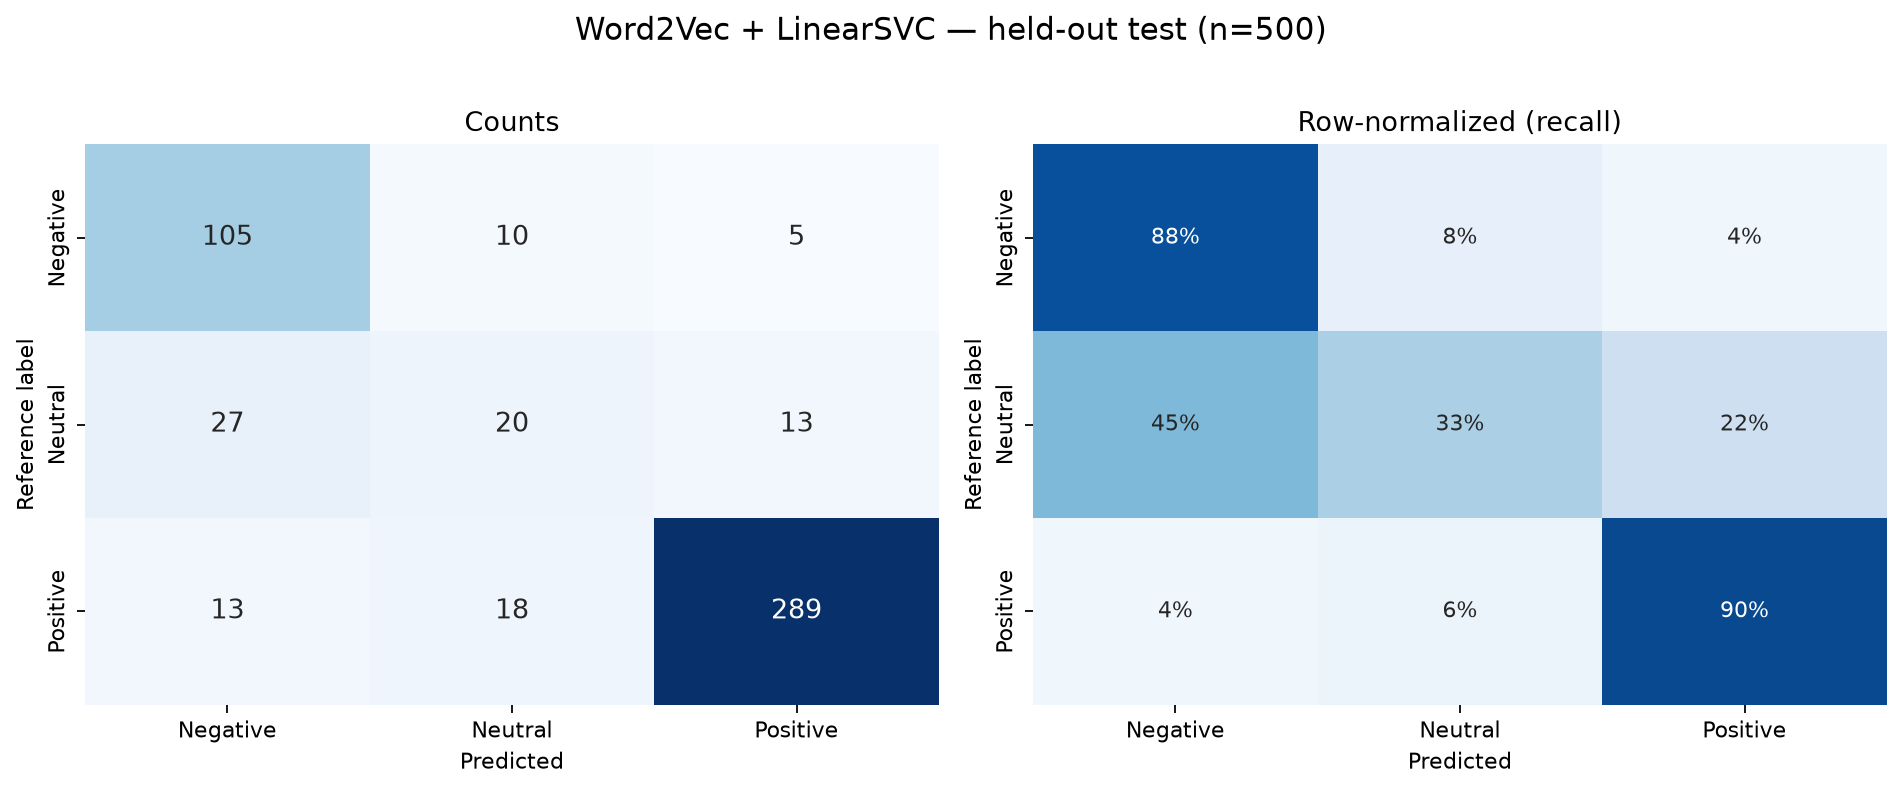
\includegraphics[width=0.95\textwidth]{cm_word2vec__linearsvc.png}
  \caption{Confusion matrix Word2Vec + LinearSVC trên held-out test (sinh từ dữ liệu Điện Máy Xanh trong repo).}
  \label{fig:cm-best}
\end{figure}

\section{Thảo luận và phân tích lỗi}
Các nhầm lẫn lớp Neutral phản ánh sự mơ hồ tự nhiên của nhiệm vụ: bình luận ``tạm ổn'', ``đẹp'', hoặc câu hỏi về sản phẩm có thể được gán khác nhau tùy ngữ cảnh và quy tắc gán nhãn. Một câu có cả lời khen dịch vụ lẫn phàn nàn về sản phẩm cũng khó rút về một nhãn cấp review. Bên cạnh đó, rating và lexicon vừa tạo target vừa quyết định trường hợp hiệu chỉnh, nên mô hình có thể học các tương quan của bộ quy tắc.

File dự đoán theo từng mẫu được lưu trong \code{outputs/predictions/word2vec__linearsvc.csv}; notebook cung cấp bảng xem lỗi theo lớp/ngành hàng để nhóm trích dẫn ví dụ sau khi rà soát. Các ví dụ nên được kiểm tra thủ công trước khi đưa nguyên văn vào bản báo cáo cuối.

\section{So sánh với mô hình Transformer}
Mã nguồn hiện hỗ trợ fine-tuning PhoBERT v2 trên văn bản đã tách từ và XLM-RoBERTa Large trên bình luận gốc, kèm weighted loss, validation Macro-F1 và early stopping. Tuy nhiên, chưa có artifact metrics Transformer trong lần chạy baseline này, vì vậy báo cáo không đưa điểm PhoBERT/XLM-R vào bảng và không khẳng định mô hình nào vượt trội. Sau khi chạy trên phần cứng phù hợp, cần bổ sung Macro-F1/per-class, confusion matrix, bootstrap interval, thời gian và cấu hình GPU; mọi mô hình phải được so sánh trên cùng split và cùng quy trình nhãn.

\section{Đe dọa tới giá trị đánh giá}
\begin{enumerate}
  \item \textbf{Pseudo-label bias:} test chưa gán độc lập; điểm số đo mức khớp với heuristic, không phải chân trị cảm xúc.
  \item \textbf{Split theo review:} cùng sản phẩm có thể xuất hiện ở train và test; kết quả có thể lạc quan nếu mô hình khai thác đặc điểm sản phẩm. Cần group split theo \code{product_code} cho đánh giá tổng quát hóa sản phẩm mới.
  \item \textbf{Mất cân bằng:} support Neutral nhỏ khiến ước lượng F1 lớp này biến động.
  \item \textbf{Lựa chọn mô hình:} các CI bootstrap chồng lấp; không nên tuyên bố ưu thế có ý nghĩa từ một lần split.
  \item \textbf{Tham số và tài nguyên:} thời gian huấn luyện cổ điển phụ thuộc môi trường; Transformer chưa được chạy nên chưa thể kết luận về trade-off chất lượng/chi phí.
\end{enumerate}
